\documentclass[11pt]{article}
\usepackage{blindtext}
\usepackage[a4paper]{geometry}
\geometry{left=1.5cm,right=1.5cm,top=1.5cm,bottom=1.5cm}
\usepackage{apacite}
\usepackage{listings}
\usepackage{amsmath, amssymb, amscd, amsthm, amsfonts, bbm, mathtools}
\usepackage{graphicx}
\usepackage{hyperref}
\usepackage{multirow}
\usepackage{booktabs} 
\usepackage{setspace}
\usepackage{threeparttable} 
\usepackage{placeins}
\usepackage[english]{babel}
\usepackage{amsthm}
\theoremstyle{definition}
\newtheorem{definition}{Definition}[section]
\usepackage{float}
% \oddsidemargin 0pt
% \evensidemargin 0pt
% \marginparwidth 40pt
% \marginparsep 10pt
% \topmargin -20pt
% \headsep 10pt
% \textheight 8.7in
% \textwidth 6.65in
\linespread{1.2}


\renewcommand{\baselinestretch}{1.0}
\bibliographystyle{apacite}
\usepackage[framed,numbered,autolinebreaks,useliterate]{mcode}
\title{Project 2 Cloud Detection}
\author{Linxuan Wang (linxuan.wang@duke.edu), Jingan Zhou (jingan.zhou@duke.edu)}

\begin{document}

\maketitle

\section{Data Collection and Exploration}
\subsection*{(a)}
Research has shown that the strongest dependences of surface air temperatures on \(CO_2\) levels will occur in the Arctic. However, Arctic-wide measurements, especially of cloud average, are required to uncover the relations fully. Cloud detection in the Arctic region is challenging given the similarity between clouds, ice, and snow, and this paper attempted to identify an accurate way to perform classification.

The data utilized in this study was collected from ten Multiangle Imaging SpectroRadiometer (MISR) orbits of path 26 over the Arctic, northern Greenland, and Baffin Bay. The time spans from April 28 through September 19, 2022. Such data is chosen due to the richness of its surface features. Each path is divided into 180 blocks, and each MISR pixel covers a \( 275 \times 275 \; m^2 \) region collected from nine cameras viewing the Earth from different angles. Five zenith angles of the cameras, 70.5° (Df), 60.0° (Cf), 45.6° (Bf), 26.1° (Af), and 0.0° (An), were included. Six data unit blocks from each orbit are included, while three of the easily identifiable ones were excluded. The author also manually extracted three features, the average linear correlation of radiation measurements at different view angles (CORR), the standard deviation of MISR nadir camera pixels across a scene (SD), and normalized difference angular index (NDAI) based on observations. Pixels were examined by experts to determine whether there is a cloud or could not decide.

The ELCM (also ELCM-QDA), SDCM, ASCM, and SVM algorithms were attempted for cloud detection. This paper showed that ELCM achieved 92\% accuracy and 100\% coverage, compared to SDCM and SACM, two previously developed MISR operational algorithms. Using this new algorithm allows us to identify clouds more accurately, which enables future studies to determine the relations to global warming.

\subsection*{(b)}
Table \ref{tab1} shows the percentage for different classes for each image and the overall result and the maps indicating classes:

\begin{table}[h]
    \centering
  \begin{tabular}{c||c|c|c|c}
	 Image
    & $1$
    & $2$
    & $3$
    & overall \\
    \hline
    \hline
    Cloud
    & 34.1\%
    & 17.8\%
    & 18.4\% 
    & 23.4\% \\
    \hline
    No Label
    & 28.6\%
    & 38.5\%
    & 52.3\%
    & 39.8\% \\
    \hline
    No Cloud
    & 37.3\%
    & 43.8\%
    & 29.3\%
    & 36.8\%
  \end{tabular}
    \caption{Data summary}
    \label{tab1}
\end{table}
\FloatBarrier

\begin{figure}[h]
\begin{minipage}[t]{0.33\textwidth}
\centering
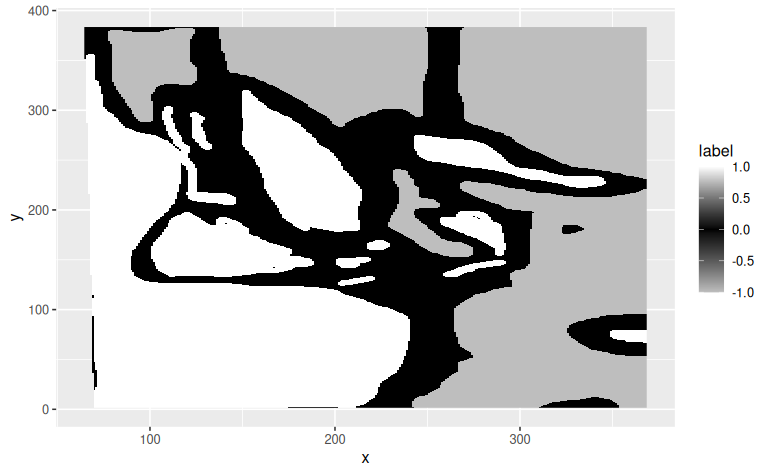
\includegraphics[width=6cm]{figures/1b1.png}
\caption{Image 1}
\label{1b1}
\end{minipage}
\begin{minipage}[t]{0.33\textwidth}
\centering
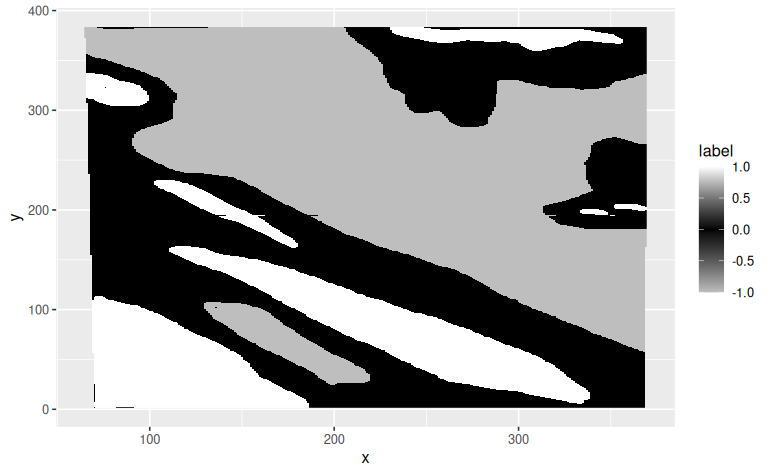
\includegraphics[width=6cm]{figures/1b2.png}
\caption{Image 2}
\label{1b2}
\end{minipage}
\begin{minipage}[t]{0.33\textwidth}
\centering
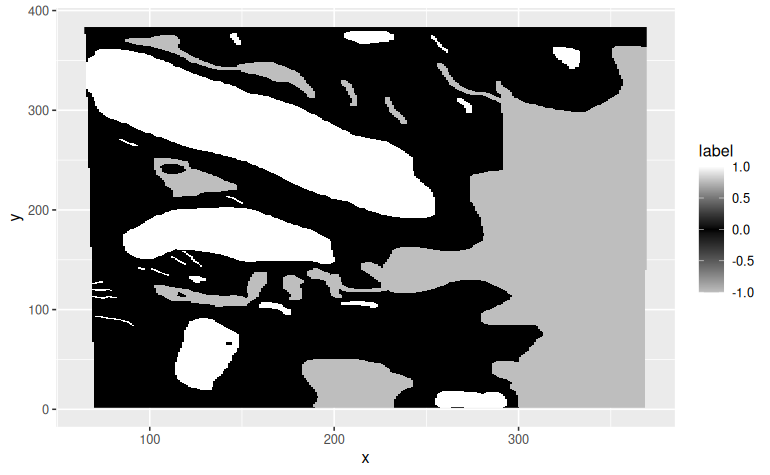
\includegraphics[width=6cm]{figures/1b3.png}
\caption{Image 3}
\label{1b3}
\end{minipage}
\end{figure}
\FloatBarrier 

Excluding those without labels, the percentages of clouds are summarized in Table \ref{tab2}:

\begin{table}[h]
    \centering
    \begin{tabular}{c||c|c|c|c}
    Image
    & $1$
    & $2$
    & $3$
    & overall \\
    \hline
    \hline
    Cloud
    & 47.8\%
    & 28.9\%
    & 38.6\% 
    & 38.9\% \\
    \hline
    No Cloud
    & 52.2\%
    & 71.1\%
    & 61.4\%
    & 61.1\%

    \end{tabular}
    \caption{Data summary after excluding invalid labels}
    \label{tab2}
\end{table}
\FloatBarrier

From the maps, we could see that:
\begin{itemize}
\item There are almost no slim slices of clouds and surfaces. Pixels with same labels tend to cluster to form large pieces of cloud or surface. This is shown in the dataset as pixels near each other tend to have the same labels unless they are at the boundaries between classes with different labels;

\item Almost no "black holes" exist in either clouds or surfaces. This pattern shows somewhat continuity of cloud and surface distribution.
\end{itemize}

Therefore, the i.i.d. assumption is not justified for the samples. Since we have observed large areas of clouds and surfaces, given a pixel in the image, in most of the scenarios it has the same label as its neighbors, which implies that pixels near each other are highly dependent and tend to have the same label.

\subsection*{(c)}

Note that from Figure 3 in the paper, we could see that the data collected for three different images consisted of roughly similar components. From the visualization in (b), we could see that the cluster pattern exists in all three images. Since the attributes for these images are similar, it makes sense to combine the attributes when performing exploratory data analysis. The correlations between features are shown in Figure \ref{1c1}.

\begin{itemize}
\item For the three imputed features (NDAI, SD, CORR), some correlation exists between SD and NDAI. The correlation between SD and CORR and that between CORR and NDAI are not as significant.

\item The correlations between NDAI, SD, CORR, and the radiance features increase as the angles decrease (from Df to An) though all the correlations are low (almost all with \(<0.5\) correlations).

\item For the radiance, we could see that the correlations between those with smaller angles are higher than those with larger angles given similar angle differences. The correlation decreases as the difference between angles increases but all correlations are at least 0.548.
\end{itemize}


\begin{figure}[h]
\centering
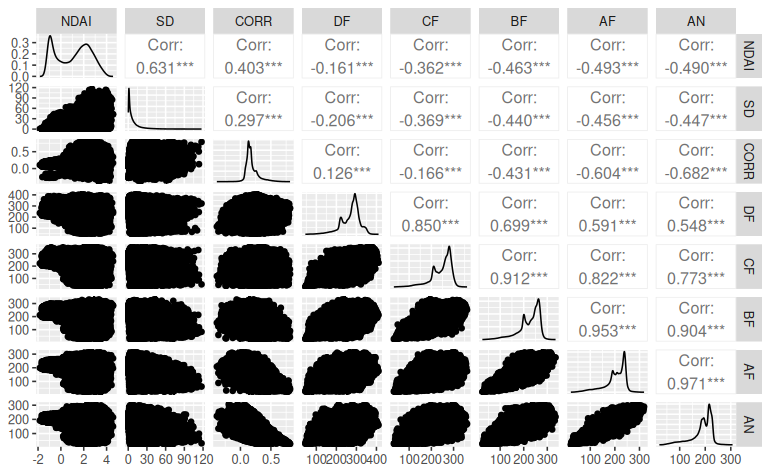
\includegraphics[width=9cm]{figures/1c1.png}
\caption{Correlations between features}
\label{1c1}
\end{figure}
\FloatBarrier

Table \ref{cor} below shows the correlation between all the features with labels. Figure \ref{1c2} and Figure \ref{1c3} demonstrate the distributions of features separated by label class.

\begin{table}[h]
    \centering
    \begin{tabular}{c||c|c|c|c|c|c|c|c|c}
    Label  & SD & NDAI & CORR & Df & Cf & Bf & Af & An \\
    \hline
    \hline
    Correlation & 0.295 & 0.617 & 0.444  & 0.007 & -0.208 & -0.338 & -0.390 & -0.389 \\

    \end{tabular}
    \caption{Correlations between labels and features}
    \label{cor}
\end{table}
\FloatBarrier

\begin{figure}[h]
\begin{minipage}[t]{0.5\textwidth}
\centering
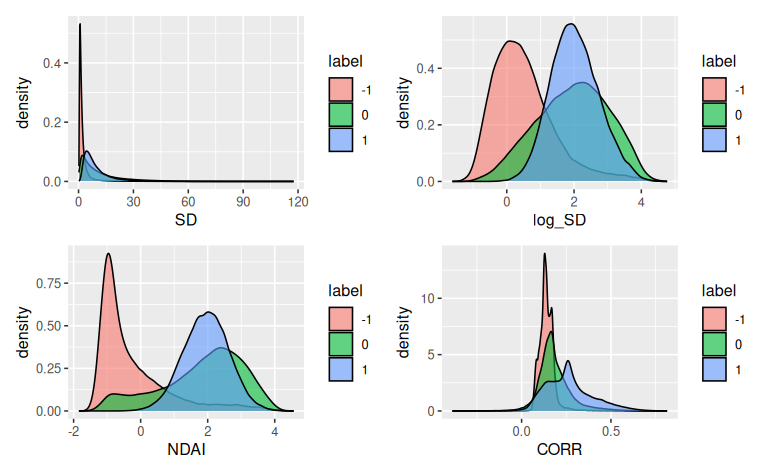
\includegraphics[width=8cm]{figures/1c2.png}
\caption{Distribution of SD, NDAI, and CORR}
\label{1c2}
\end{minipage}
\begin{minipage}[t]{0.5\textwidth}
\centering
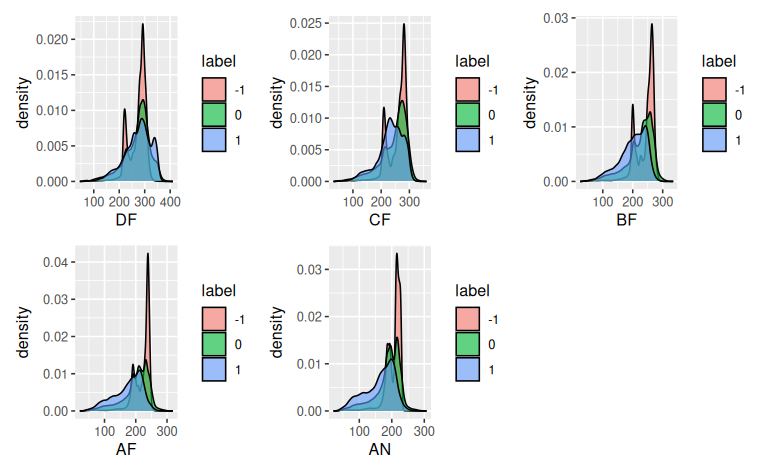
\includegraphics[width=9cm]{figures/1c3.png}
\caption{Distribution from five zenith angles}
\label{1c3}
\end{minipage}
\end{figure}
\FloatBarrier 

\begin{itemize}
\item For the three essential engineered features (SD, NDAI, CORR): samples labeled ``no cloud'' typically have lower SD, NDAI, and CORR. Also, almost all data points with low NDAI are labeled as ``no cloud'', while a few are undetermined and almost none are labeled as "cloud".

\item For the five radiance features: samples labeled "no cloud" typically have two peaks, and are more tightly distributed. Samples labeled ``cloud'' are more sparsely distributed and negatively skewed. The peak for samples labeled ``cloud'' normally lies between the peaks for samples labeled "no cloud". The correlations between labels and these features are low and most are negatively correlated.
\end{itemize}


\section{Preparation}
\subsection*{(a)}
Cross-validation is a resampling method that uses different portions of the data to test and train a model on different iterations. It is widely applied when people are not allowed to touch the test data. In a scenario where i.i.d. assumption is justified for the dataset, we can simply randomly split the dataset into several non-overlapping groups. Each group acts as a validation set and the remainder as a training set. However, in a scenario where i.i.d. assumption is not justified, we can't apply this simple split method. The reason is that those non-overlapping groups may be close to each other. We first use a plot to illustrate the ``closeness'' here, then we explain why this matters.
\begin{figure}[h]
\small
\centering
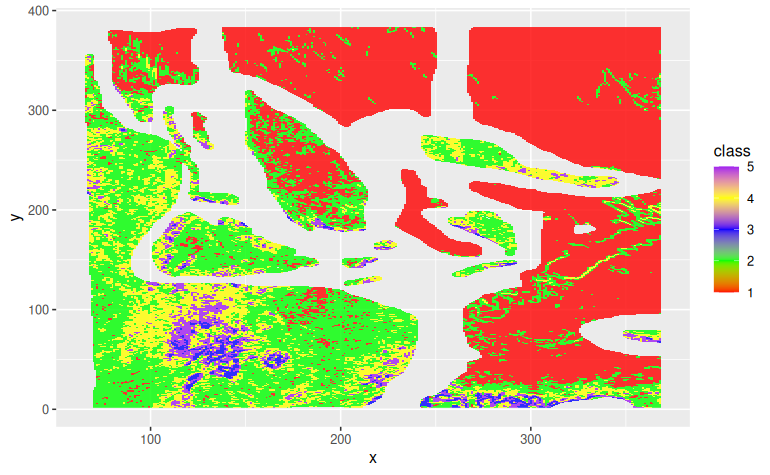
\includegraphics[width=7cm]{figures/2a1.png}
\caption{Undesirable split method}
\label{2a1}
\end{figure}
\FloatBarrier

We split the dataset into five groups using an undesirable method and show the results in Figure \ref{2a1}. We can see that pixels from all groups scattered at the bottom-left part of the plot. This pattern destroys the power of cross-validation in a way that, if we choose Group 5 (which is colored in purple) as the validation set, most of the pixels in the validation set can be approximated by a pixel in the training set. In this case we say that the validation set is "closed" to the training set. Because of the strong spatial dependency, pixels near each other tend to have the same labels and similar features. Therefore, we can design a naive classifier taking advantage of the closeness: for each pixel, $x_i$ in the validation set, find the pixel $x_i'$ in the training set and assign it to $x_i$. This naive classifier should be performing well under cross-validation, but actually has a poor generalization ability because we are no longer able to find pixels in the training set that approximate pixels in new images. As a result, cross-validation error is no longer a good proxy for test error. 

To take the fact that data is not i.i.d. into account, we would like to split the image into several "blocks" that are treated as sub-images, such that each block only borders other blocks at the boundary. This data splitting method significantly reduces the similarity/closeness between the training set and validation set as well as the testing set. In the meantime, we want each sub-image contains a fair amount of pixels of clouds and surfaces to achieve better performances. Note that the second condition is not easy to satisfy later in the \textbf{CVmaster} function. Here, we introduce two general split methods to create the blocks. We showcase why those two methods work by applying them to our dataset. 

\subsubsection*{Method I -- $K$-Means}
The first one is inspired by $K$-Means clustering. $K$-Means clustering automatically splits the whole dataset into $K$ groups such that samples within each group are similar to each other. Our first method performs $K$-Means clustering, where $K=5$, on each of the images based on $x$ and $y$ coordinates. In this way, we have 15 sub-images in total. Furthermore, we manually select 9 of them as the training set, 3 of them as the validation set, and 3 of them as the testing set. Again, note that it is not easy to include this manual selection process in the \textbf{CVmaster} function, so we skip this second step later when designing the function. The split result is shown in Figure \ref{2a2}, \ref{2a3}, \ref{2a4}. The manual selection rule is shown in Table \ref{tab3}

\begin{figure}[h]
\begin{minipage}[t]{0.33\textwidth}
\centering
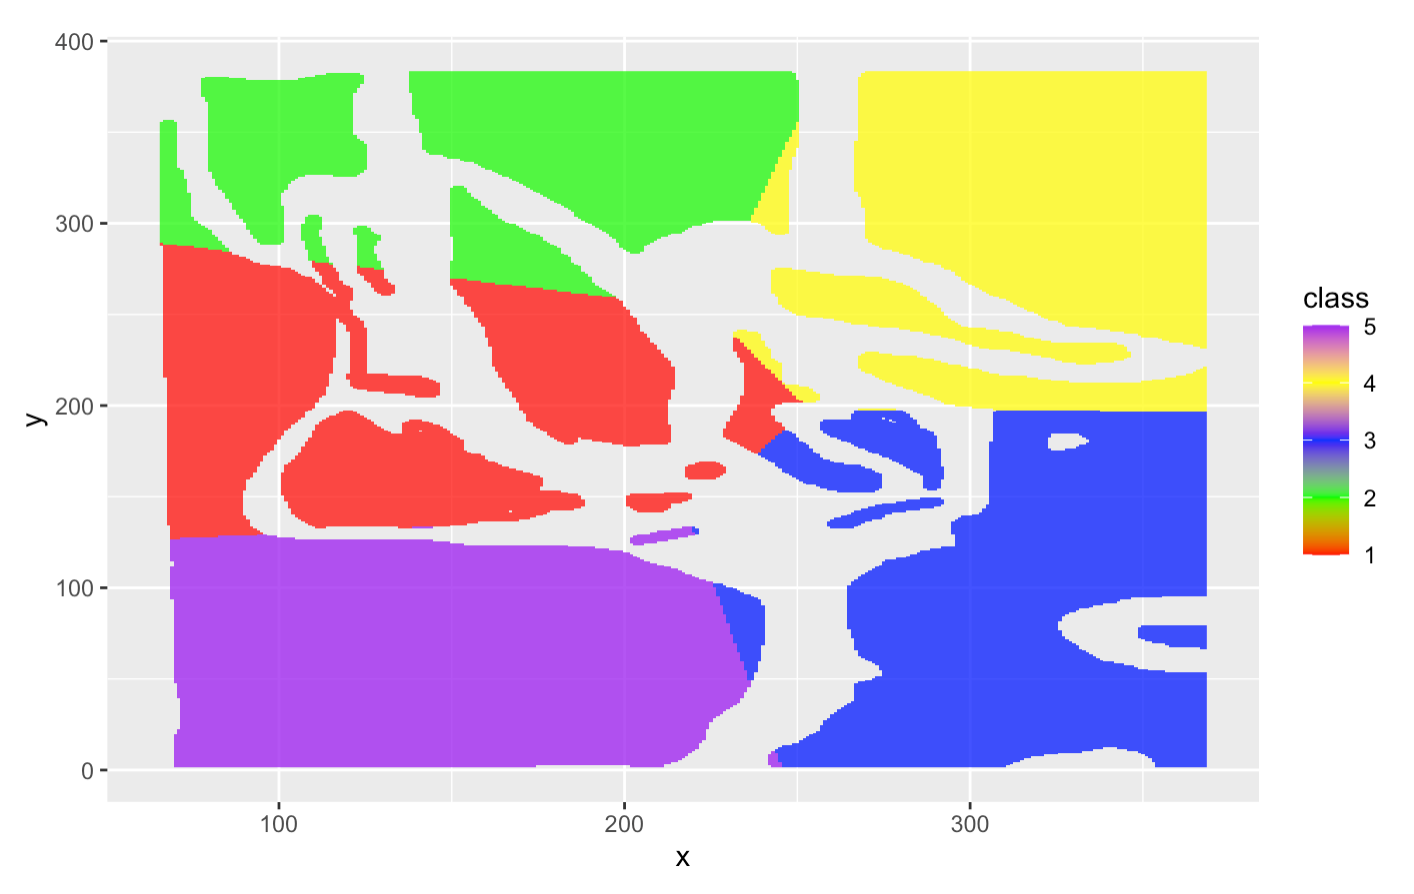
\includegraphics[width=5cm]{figures/2a2.png}
\caption{Image 1}
\label{2a2}
\end{minipage}
\begin{minipage}[t]{0.33\textwidth}
\centering
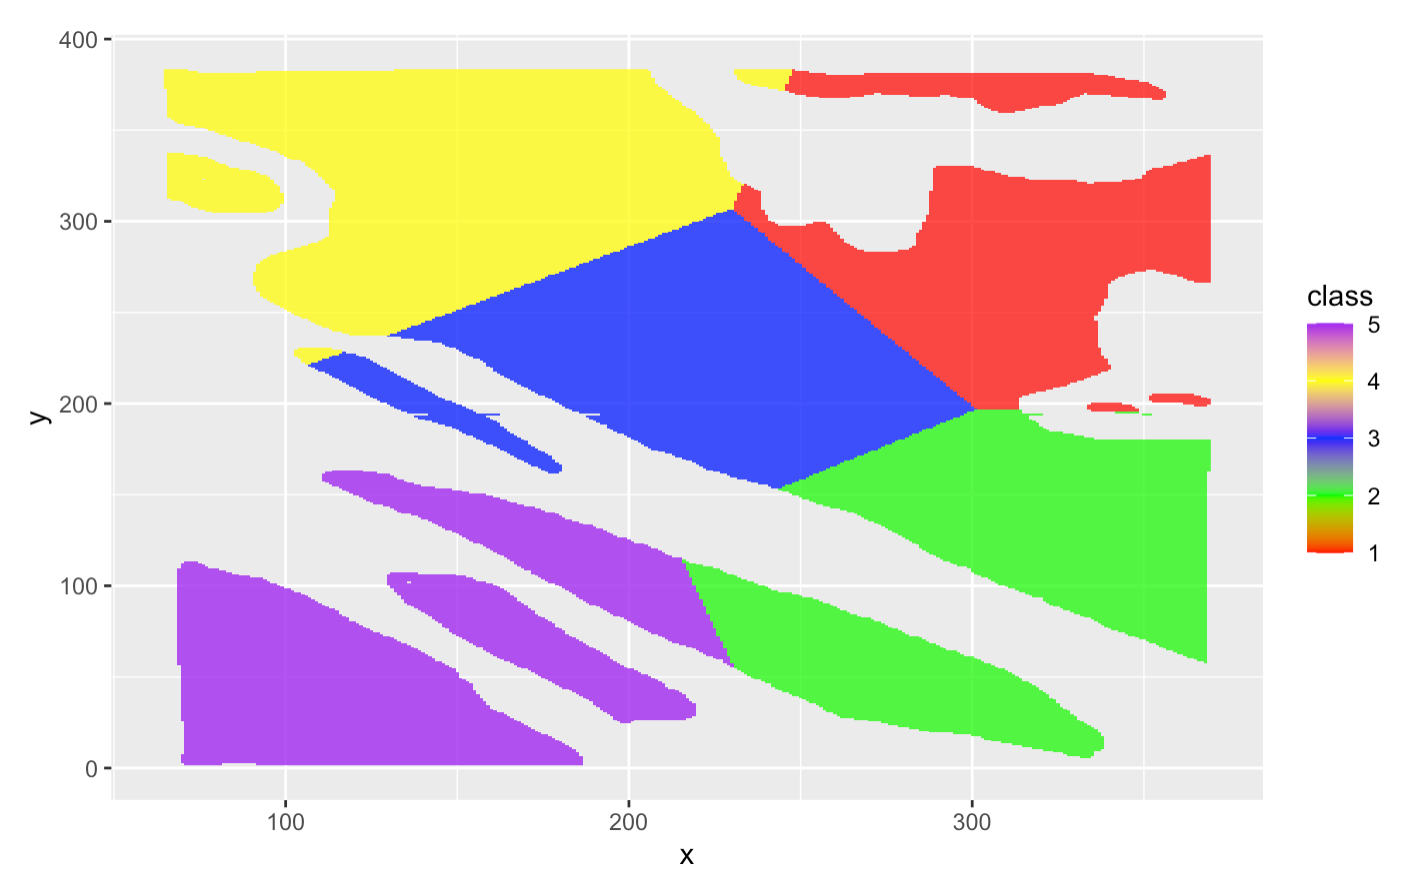
\includegraphics[width=5cm]{figures/2a3.png}
\caption{Image 2}
\label{2a3}
\end{minipage}
\begin{minipage}[t]{0.33\textwidth}
\centering
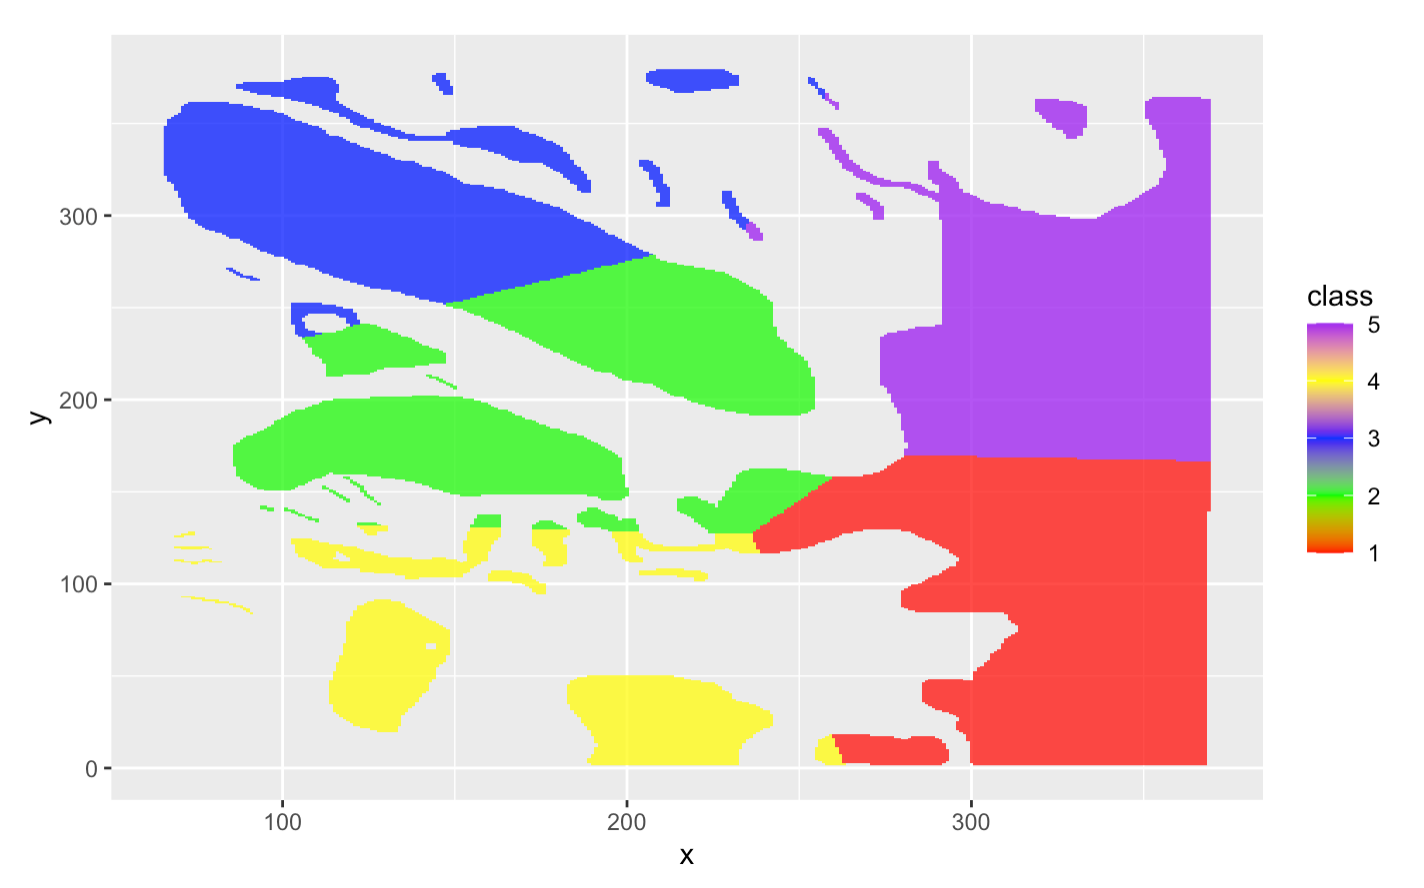
\includegraphics[width=5cm]{figures/2a4.png}
\caption{Image 3}
\label{2a4}
\end{minipage}
\end{figure}
\FloatBarrier 

\begin{table}[h]
    \centering
    \begin{tabular}{c||c|c|c||c}
    Image
    & $1$
    & $2$
    & $3$ 
    &\\
    \hline
    \hline
    Blocks to training/\#-1:\#1 in training set
    & 2,4,5
    & 2,4
    & 1,2,3,4 
    & 71998:50565\\
    \hline
    Blocks to validation/\#-1:\#1 in validation set
    & 3
    & 1,5
    & None 
    & 28514:14740\\
    \hline
    Blocks to testing/\#-1:\#1 in testing set 
    & 1
    & 3
    & 5
    & 26568:15676

    \end{tabular}
    \caption{Block assignment and number of labels in each set}
    \label{tab3}
\end{table}
\FloatBarrier

\subsubsection*{Method II -- Vertical Split}
The second method is named ``Vertical Split''. For each image, we simply divide the image into 5 sub-images vertically, each of which contains approximately one-fifth of pixels of the whole image. Then we look into all the 15 sub-images and manually assign them to the training, validation, and testing set. Visualization and manual assignment is displayed in Figure Figure \ref{2a5}, \ref{2a6}, \ref{2a7} and Table \ref{tab4}.

\begin{figure}[h]
\begin{minipage}[t]{0.33\textwidth}
\centering
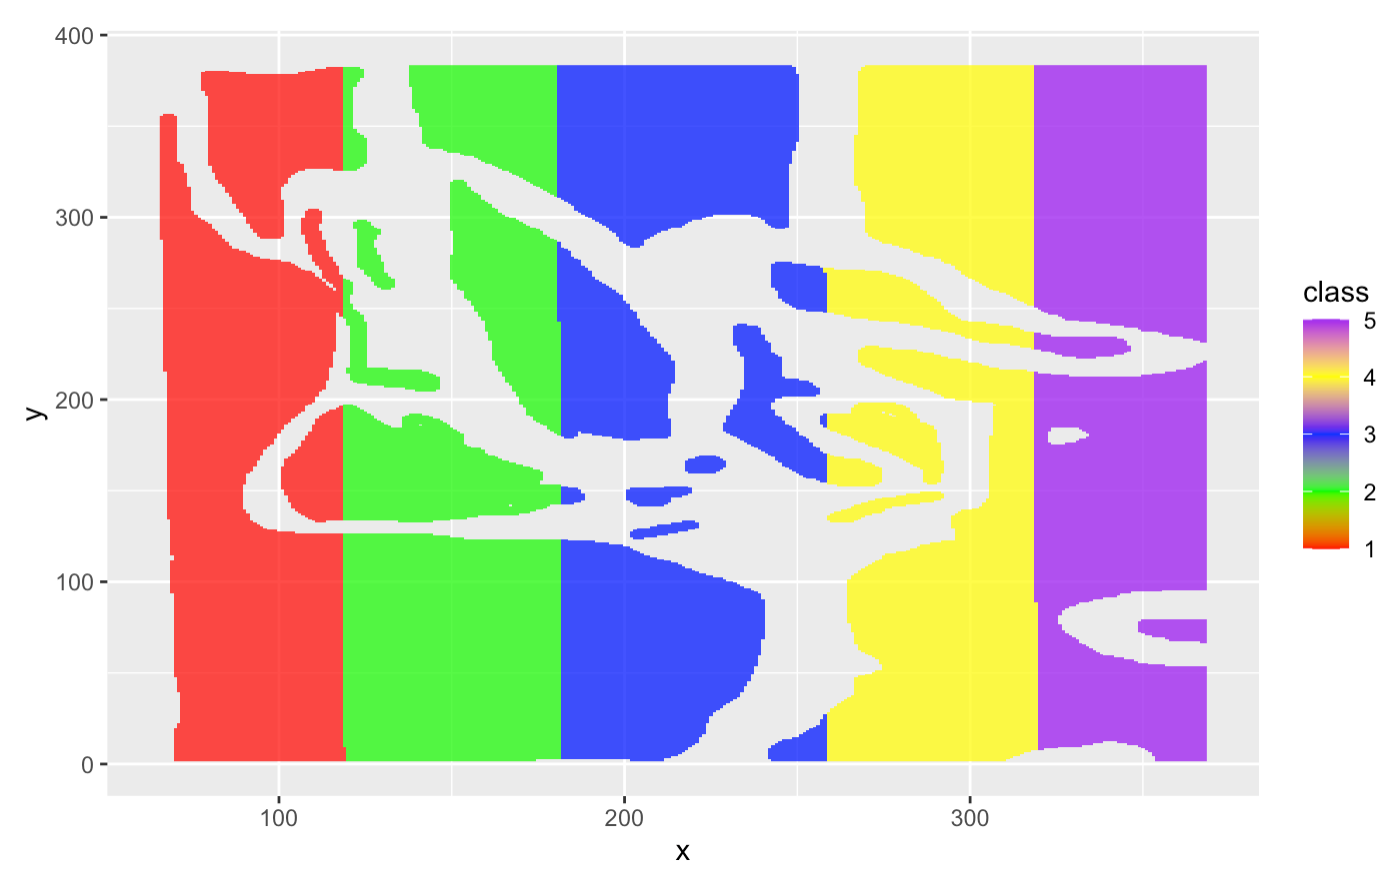
\includegraphics[width=5cm]{figures/2a5.png}
\caption{Image 1}
\label{2a5}
\end{minipage}
\begin{minipage}[t]{0.33\textwidth}
\centering
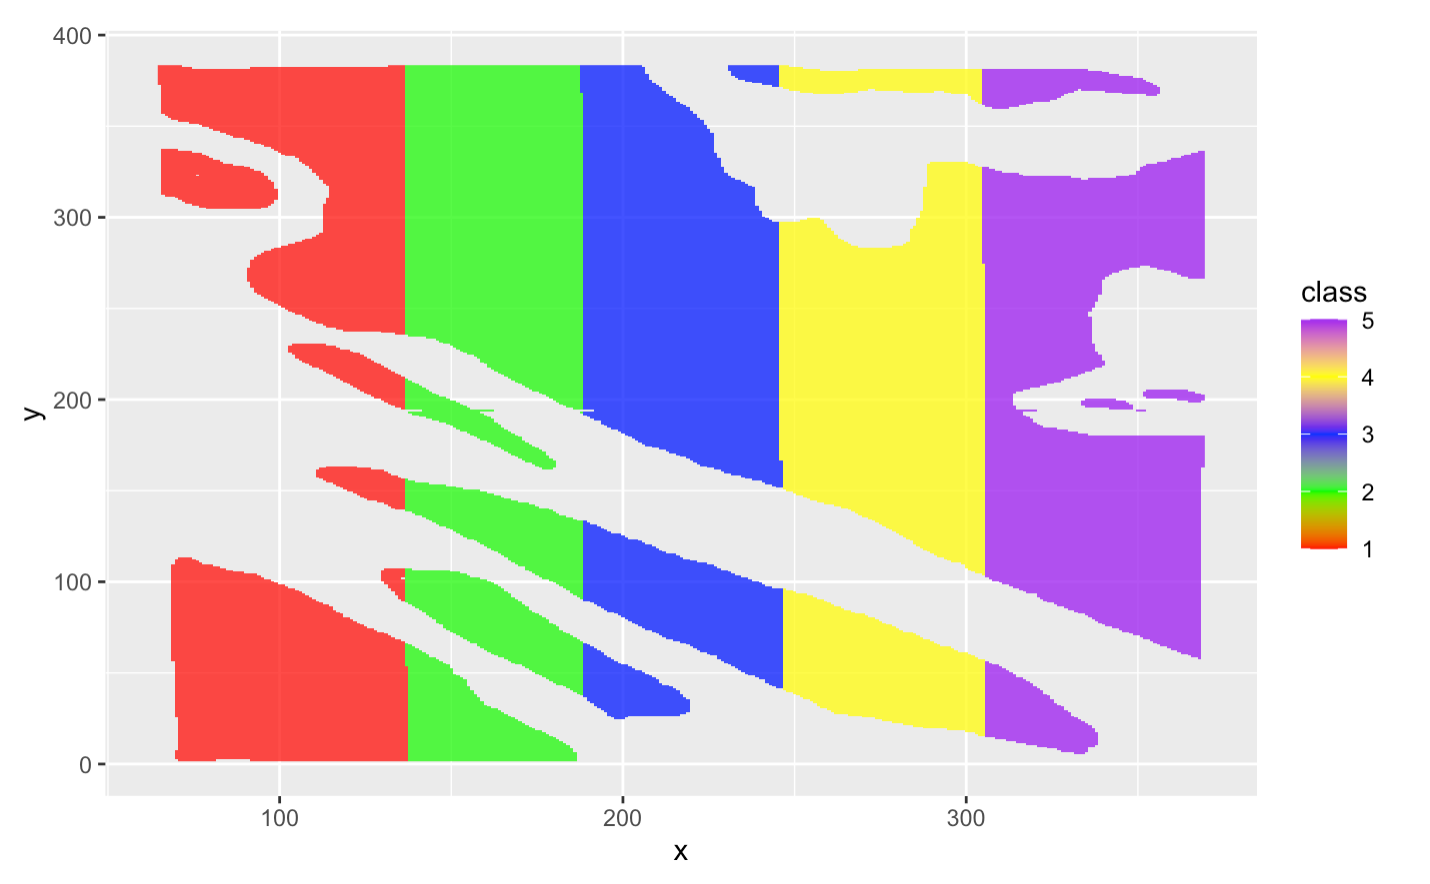
\includegraphics[width=5cm]{figures/2a6.png}
\caption{Image 2}
\label{2a6}
\end{minipage}
\begin{minipage}[t]{0.33\textwidth}
\centering
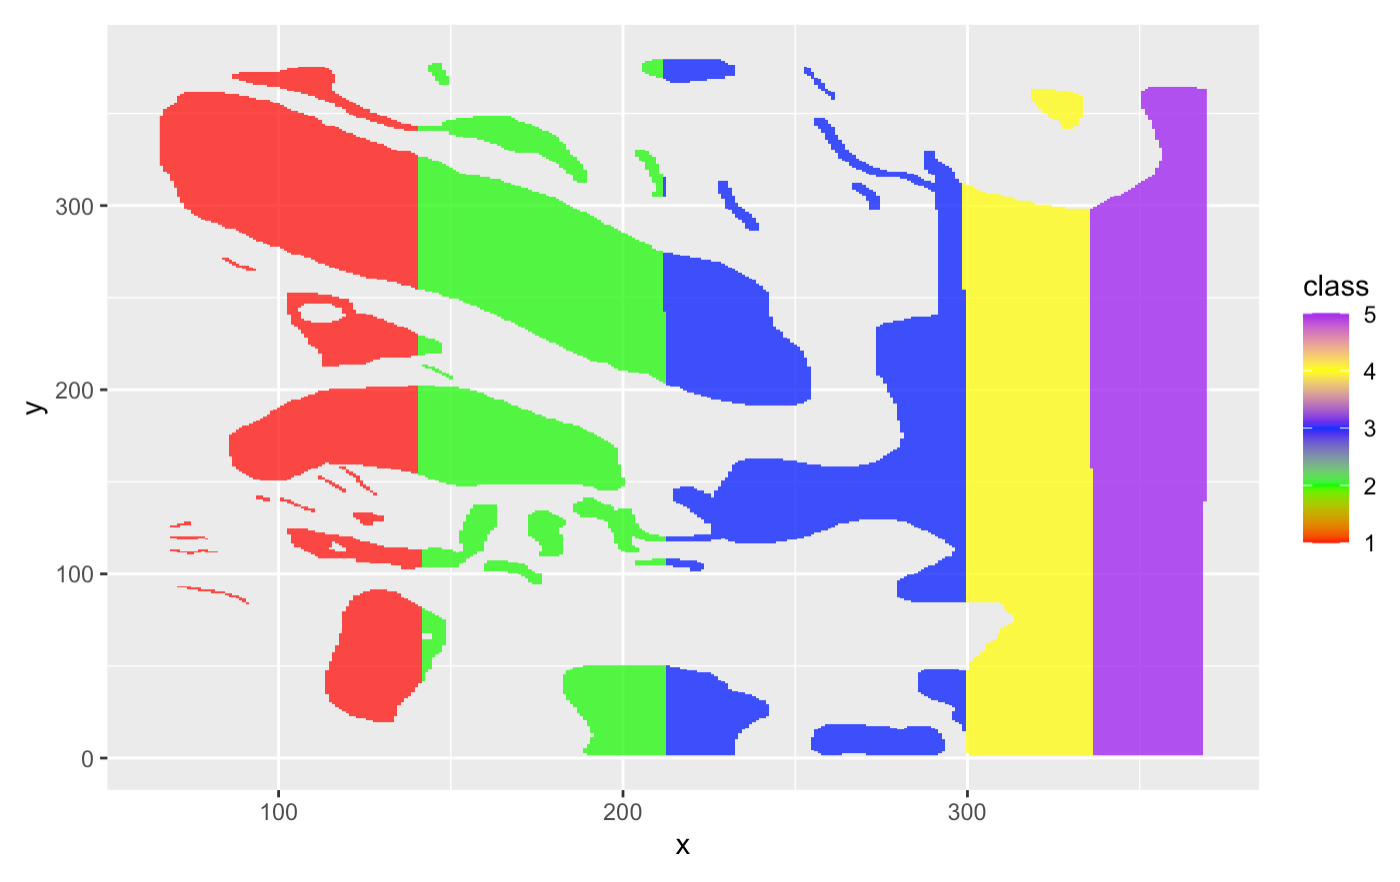
\includegraphics[width=5cm]{figures/2a7.png}
\caption{Image 3}
\label{2a7}
\end{minipage}
\end{figure}
\FloatBarrier 

%\begin{center}
\begin{table}[h]
    \centering
    \begin{tabular}{c||c|c|c||c}
    Image
    & $1$
    & $2$
    & $3$ 
    &\\
    \hline
    \hline
    Blocks to training/\#-1:\#1 in training set
    & 3,4,5
    & 1,4
    & 1,2,3,5 
    & 77812:44470\\
    \hline
    Blocks to validation/\#-1:\#1 in validation set
    & 2
    & 2,5
    & None 
    & 25214:19583\\
    \hline
    Blocks to testing/\#-1:\#1 in testing set 
    & 1
    & 3
    & 4
    & 24684:16928

    \end{tabular}
%\end{center}
    \caption{Block assignment and number of labels in each set}
    \label{tab4}
\end{table}
\FloatBarrier



 

\subsection*{(b)}
The accuracy of the trivial classifier is reported in Table \ref{tab5}.
\begin{table}[h]
    \centering
    \begin{tabular}{c||c|c}
    
    & Validation
    & Test\\
    \hline
    \hline
    $K$-Means Split
    & 0.659
    & 0.563\\
    \hline
    Vertical Split
    & 0.629
    & 0.593

    \end{tabular}
%\end{center}
    \caption{Accuracy of trivial classifier}
    \label{tab5}
\end{table}
\FloatBarrier
It is easy to see that this classifier has higher accuracy when there is almost no cloud in the image.

\subsection*{(c)}
We would like to examine the distributions of features conditional on labels. Our criteria for ``best'' features is based on a conjecture that the overlapping area of orange and blue region in Figure \ref{1c2}, \ref{1c3} should be the smallest for the ``best'' feature. EDA in Question 1 suggests that log\_SD, NDAI, and CORR may be the three ``best'' features. This is also inspired by the original paper where authors find thresholds for three engineered features and assign labels based on that. We define our criteria \textbf{F}eature-\textbf{P}ower-of-\textbf{C}lassification mathematically and find our three ``best'' features.

\begin{definition}[FPC]

For a dataset containing feature $x^i$ and label $y$, $y \in \{-1,1\}$. Let $\hat{F}^i_{-1}$ and $\hat{F}^i_1$ denote the empirical c.d.f. of $x^i$ given $y=-1$ and $y=1$, respectively. $\text{FPC}_i$ of feature $x^i$ is defined as 
$$
\text{FPC}_i = \max\{ \max_x\hat{F}^i_{-1}(x)+1-\hat{F}^i_{1}(x),\max_x\hat{F}^i_{1}(x)+1-\hat{F}^i_{-1}(x) \}.
$$
Equivalently, it can be defined as
$$
\text{FPC}_i = 1 + \max_x |\hat{F}^i_{-1}(x)-\hat{F}^i_{1}(x)|
$$

\end{definition}

Intuitively, FPC measures the maximum non-overlapping area of two conditional densities. The results are as in Table \ref{tab6}.

\begin{table}[h]
    \centering
    \begin{tabular}{c||c|c|c|c|c|c|c|c}
     
    & NDAI
    & SD
    & CORR
    & DF
    & CF
    & BF
    & AF
    & AN \\
    \hline
    \hline
    FPC
    & 1.875
    & 1.722
    & 1.899
    & 1.466
    & 1.356
    & 1.587
    & 1.664
    & 1.614

    \end{tabular}
%\end{center}
    \caption{FPC of features}
    \label{tab6}
\end{table}
\FloatBarrier

Indeed, NDAI, SD, and CORR are the three ``best'' features.

\subsection*{(d)}
Our \textbf{CVmaster} function supports 6 classifiers: Logistic Regression, Linear Discriminant Analysis, Quadratic Discriminant Analysis, Naive Bayes, Random Forest, and XGBoost. Users can select the classifier by passing one of \{``Logistic'',``LDA'',``QDA'',``naiveBayes'',``randomForest'',``xgboost''\} to the argument \texttt{classifier}. Training features, labels, and coordinates can be passed to \texttt{features}, \texttt{labels}, and \texttt{coordinate}, respectively. \textbf{CVmaster} sets the default number of cross-validation folds at 10, while users can also select other number by passing to the argument \texttt{K}. Besides, users can choose the folds split method from \{folds.Kmeans, folds.Vsplit\}, which are two auxiliary functions that are included in our code. Arguments \texttt{tree.num}, \texttt{tree.depth} and \texttt{eta} are hyperparameters for classifiers Random Forest and XGBoost. \textbf{CVmaster} will do a grid search on those hyperparameters and return the best values. More detailed usage is included in the function documentation.



\section{Modeling}
\subsection*{(a)}
We attempt 6 different classification methods to detect clouds and their respective assumptions are listed below. 
\begin{itemize}
\item \textbf{Logistics Regression:} It assumes \( Y_i|X_i \sim \text{Bernoulli}\Big(\dfrac{e^{x_i^T \beta}}{1+e^{x_i^T \beta}}\Big)\) where \(Y_i's\) the response variables are conditionally independent given \(X_i's\). It also assumes independent observations and no multicollinearity. From Figure \ref{1c1}, there might be minor multicollinearity issues as Bf, Af, and An are highly correlated with most correlations \( > 0.9\). Also, previous analysis has shown the existence of spatial dependence, so the assumptions for logistics regressions are not all satisfied.

\item \textbf{Linear Discriminant Analysis (LDA):} It assumes multivariate normality (i.e., independent variables are normal for each label) and homoscedasticity (i.e., variances and covariances among group variables are the same across labels). It also assumes independent observations and no multicollinearity. In Figure \ref{1c3}, we see that some features are bimodal and hence the normality assumption is not satisfied.

\item \textbf{Quadratic Discriminant Analysis (QDA):} Same assumption as LDA except that we do not assume the same covariances among group variables. The normality assumption is not satisfied here as well.

\item \textbf{Naive Bayes:} It assumes that the presence of one feature in a label is unrelated to the presence of any other feature. Since all features are correlated and some are highly correlated with correlations \( > 0.7\), the conditional independence assumption is not satisfied.

\item \textbf{Random Forest:} The data does not contain any missing value and hence the assumption is satisfied. The predictions from each tree must have low correlations.

\item \textbf{Extreme Gradient Boosting (XGBoost):} It does not make any independence or distributional assumption. This model would undergo additive training through a sequential procedure, and then shrinkage and feature sub-sampling would be used to prevent overfitting.
\end{itemize}

For methods that require hyperparameter tunings such as Random Forest and XGBoost, we perform a grid search to identify the optimal models. The classification errors are summarized in Table \ref{CVK} and Table \ref{CVV}. Note that the optimal Random Forests selected for $K$-means splitting methods have 600 trees with a depth of 15, and for Vertical Split methods have 550 trees with a depth of 15. For XGboost, the optimal tree depth is 3 for both methods, while eta is 0.4 for $K$-means and 0.3 for the vertical split. Grid for Random Forest is $\texttt{seq(200,600,50)}\times\texttt{seq(5,15,1)}$.  The cross-validation errors are shown in Table \ref{CVK} and \ref{CVV}, while the test errors are in Table \ref{Test}.

\begin{table}[h]
    \centering
    \begin{tabular}{c||c|c|c|c|c|c|c|c|c|c|c}
    Algorithm & Fold 1 & 2 & 3 & 4 & 5 & 6 & 7 & 8 & 9 & 10 & Average \\
    \hline
    \hline
    Logistic Regression & 0.11 & 0.08 & 0.03 & 0.01 & 0.32 & 0.33 & 0.00 & 0.29 & 0.02 & 0.00 & 0.119 \\
    \hline
    LDA & 0.10 & 0.06 & 0.03 & 0.01 & 0.21 & 0.35 & 0.03 & 0.28 & 0.01 & 0.00 & 0.107 \\
    \hline
    QDA & 0.11 & 0.09 & 0.01 & 0.00 & 0.13 & 0.28 & 0.00 & 0.34 & 0.01 & 0.00 & 0.097 \\
    \hline
    Naive Bayes & 0.22 & 0.02 & 0.00 & 0.00 & 0.44 & 0.48 & 0.00 & 0.51 & 0.00 & 0.00 & 0.170 \\
    \hline
    Random Forest & 0.09 & 0.05 & 0.03 & 0.00 & 0.40 & 0.32 & 0.01 & 0.24 & 0.00 & 0.00 & 0.116 \\
    \hline
    XGBoost & 0.07 & 0.05 & 0.01 & 0.01 & 0.47 & 0.42 & 0.01 & 0.27 & 0.00 & 0.00 & 0.132

    \end{tabular}
    \caption{CV Classification Errors for $K$-means Split}
    \label{CVK}
\end{table}
\FloatBarrier

\begin{table}[h]
    \centering
    \begin{tabular}{c||c|c|c|c|c|c|c|c|c|c|c}
    Algorithm & Fold 1 & 2 & 3 & 4 & 5 & 6 & 7 & 8 & 9 & 10 & Average \\
    \hline
    \hline
    Logistic Regression & 0.11 & 0.12 & 0.16 & 0.15 & 0.14 & 0.17 & 0.13 & 0.10 & 0.06 & 0.06 & 0.119 \\
    \hline
    LDA & 0.04 & 0.19 & 0.02 & 0.32 & 0.18 & 0.09 & 0.00 & 0.00 & 0.16 & 0.11 & 0.112 \\
    \hline
    QDA & 0.03 & 0.16 & 0.01 & 0.27 & 0.17 & 0.14 & 0.01 & 0.00 & 0.19 & 0.14 & 0.111 \\
    \hline
    Naive Bayes & 0.04 & 0.07 & 0.09 & 0.11 & 0.09 & 0.12 & 0.11 & 0.14 & 0.11 & 0.11 & 0.099 \\
    \hline
    Random Forest & 0.06 & 0.06 & 0.12 & 0.07 & 0.06 & 0.10 & 0.06 & 0.06 & 0.03 & 0.05 & 0.069 \\
    \hline
    XGBoost & 0.05 & 0.10 & 0.11 & 0.12 & 0.10 & 0.14 & 0.08 & 0.07 & 0.07 & 0.08 & 0.092

    \end{tabular}
    \caption{CV Classification Errors for Vertical Split}
    \label{CVV}
\end{table}
\FloatBarrier

\begin{table}[h]
    \centering
    \begin{tabular}{c||c|c|c|c|c|c}
    Test Set & Logistic Regression
    & LDA
    & QDA & Naive Bayes & Random Forest & XGBoost \\
    \hline
    \hline
    $K$-Means Split
    & 0.945 & 0.843 & 0.887 & 0.921 & 0.888 & 0.892\\
    \hline
    Vertical Split
    & 0.959
    & 0.908 & 0.930 & 0.839 & 0.956 & 0.930

    \end{tabular}
%\end{center}
    \caption{Test Accuracy}
    \label{Test}
\end{table}
\FloatBarrier

\subsection*{(b)}
The ROC curves for $K$-means and vertical split for all the algorithms are shown in Figure \ref{3bK} and \ref{3bV}.

Generally, we might not put equal weights on specificity and sensitivity as they might have different effects on the outcomes. In our case, a false negative represents not detecting a cloud when there is a cloud, while a false positive indicates identifying a cloud without a cloud. Both directions are quite costly as they would all further affect other estimates such as surface temperature. In other words, we emphasize both false negative rate and false positive rate equally and we would like to maximize total sensitivities and specificities. The thresholds are summarized in Table \ref{threshold}.

From the ROC curves, we could see that the performance of logistic regression and random forest are relatively good and stable in both splitting methods. LDA and QDA perform quite well in the $K$-means splitting test set but not quite in the vertical splitting test set. Naive Bayes and XGBoost provide relatively low error rates in the vertical splitting test set but are the worst in the $K$-means splitting test set.

\begin{figure}[h]
\begin{minipage}[t]{0.5\textwidth}
\centering
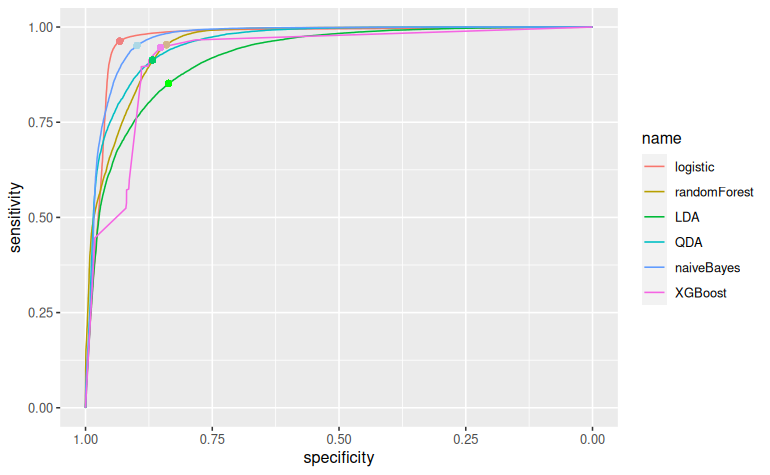
\includegraphics[width=8.5cm]{figures/3bK.png}
\caption{ROC curves for K-mean split}
\label{3bK}
\end{minipage}
\begin{minipage}[t]{0.5\textwidth}
\centering
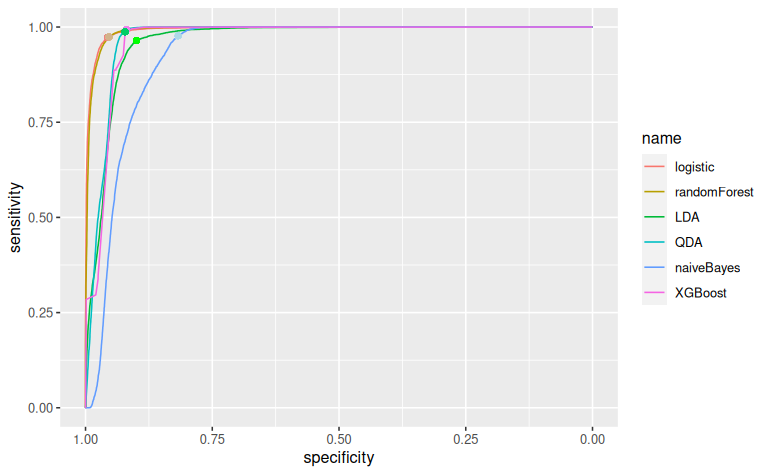
\includegraphics[width=8.5cm]{figures/3bV.png}
\caption{ROC curves for vertical split}
\label{3bV}
\end{minipage}
\end{figure}
\FloatBarrier 

\begin{table}[h]
    \centering
    \begin{tabular}{c||c|c|c|c|c|c}
    Test Set & Logistic Regression
    & LDA
    & QDA & Naive Bayes & Random Forest & XGBoost \\
    \hline
    \hline
    $K$-Means Split
    & 0.359 & 0.278 & 0.013 & 0.047 & 0.260 & 0.290\\
    \hline
    Vertical Split
    & 0.129
    & 0.181 & 0.013 & 0.000329 & 0.580 & 0.481

    \end{tabular}
%\end{center}
    \caption{Cutoff values for algorithms}
    \label{threshold}
\end{table}
\FloatBarrier

\subsection*{(c)}
Some other metrics that could be considered include:

\begin{itemize}
\item \textbf{Negative Prediction Value (NPV) and Positive Prediction Value (PPV):} The proportions of positive and negative results that are true positive and true negative results, respectively. These results also take prevalence into account, meaning that they would be more suitable for a relatively balanced data set. Hence, these are indeed useful metrics in our case.

\item \textbf{F1 score:} defined as \( 2 \times \dfrac{\text{PPV}\cdot \text{Sensitivity}}{\text{PPV} + \text{Sensitivity}}\), i.e., it combines sensitivity and PPV into a single metric by taking their harmonic mean.
\end{itemize}


Here we present the PPV, NPV, and F1 score information in Table \ref{metricsK} and \ref{metricsV}. We could indeed see that the values for NPV are all higher than those for PPV. This is reasonable as there are more pixels labeled as "no cloud". Also, compared with the values from the $K$-mean split, NPVs are higher and PPVs are significantly lower than those from vertical splits. 

We then compare the F1 scores across models as the scores incorporate two important metrics and both of which are suitable for our analysis. Logistic Regression has the highest F1 score, followed by Random Forest, QDA, and XGBoost, LDA. The F1 score for Naive Bayes is not stable as it has a low PPV score for the vertical split. 

\begin{table}[h]
    \centering
    \begin{tabular}{c||c|c|c|c|c|c}
    $K$-means Split & Logistic Regression & LDA & QDA & Naive Bayes & Random Forest & XGBoost \\
    \hline
    \hline
    NPV
    & 0.972 & 0.887 & 0.933 & 0.962 & 0.961 & 0.957 \\
    \hline
    PPV
    & 0.912
    & 0.790 & 0.833 & 0.871 & 0.812 & 0.822 \\
    \hline
    F1 score
    & 0.937 & 0.820 & 0.872 & 0.910 & 0.877 & 0.880
    \end{tabular}
%\end{center}
    \caption{NPV, PPV, F1 score for $K$-means split}
    \label{metricsK}
\end{table}
\FloatBarrier


\begin{table}[h]
    \centering
    \begin{tabular}{c||c|c|c|c|c|c}
     Vertical Split & Logistic Regression & LDA & QDA & Naive Bayes & Random Forest & XGBoost \\
    \hline
    \hline
    NPV
    & 0.996 & 0.994 & 0.999 & 0.996 & 0.996 & 0.998 \\
    \hline
    PPV
    & 0.780
    & 0.603 & 0.662 & 0.459 & 0.769 & 0.667 \\
    \hline
    F1 score
    & 0.866 & 0.742 & 0.794 & 0.625 & 0.860 & 0.796
    \end{tabular}
%\end{center}
    \caption{NPV, PPV, F1 score for vertical split}
    \label{metricsV}
\end{table}
\FloatBarrier

\section{Diagnostics}
After training all the classifiers and examining their results, we find a noteworthy phenomenon: classification accuracy largely depends on how we design the training and testing (validation) dataset. Looking back at Table \ref{CVK} and \ref{CVV} we can find that there are several folds (e.g., Fold 6,8 under $K$-Means Split and Fold 4 under Vertical Split) on which all the classifiers perform badly. 

In this section, we conduct an in-depth analysis of the Random Forest classifier since it performs well under both split methods according to our CV errors, and CV error best measures a classifier's generalization ability. That is also why we do not choose Logistic Regression as our best classifier. All analyses are done on the training and testing dataset split by the Vertical Split method. 

\subsection*{(a)}
We first fix the depth of trees at 15 and plot test error against the number of trees in Figure \ref{TCE}. The cutoff value is automatically selected by the \texttt{ranger} function.

\begin{figure}[h]
\small
\centering
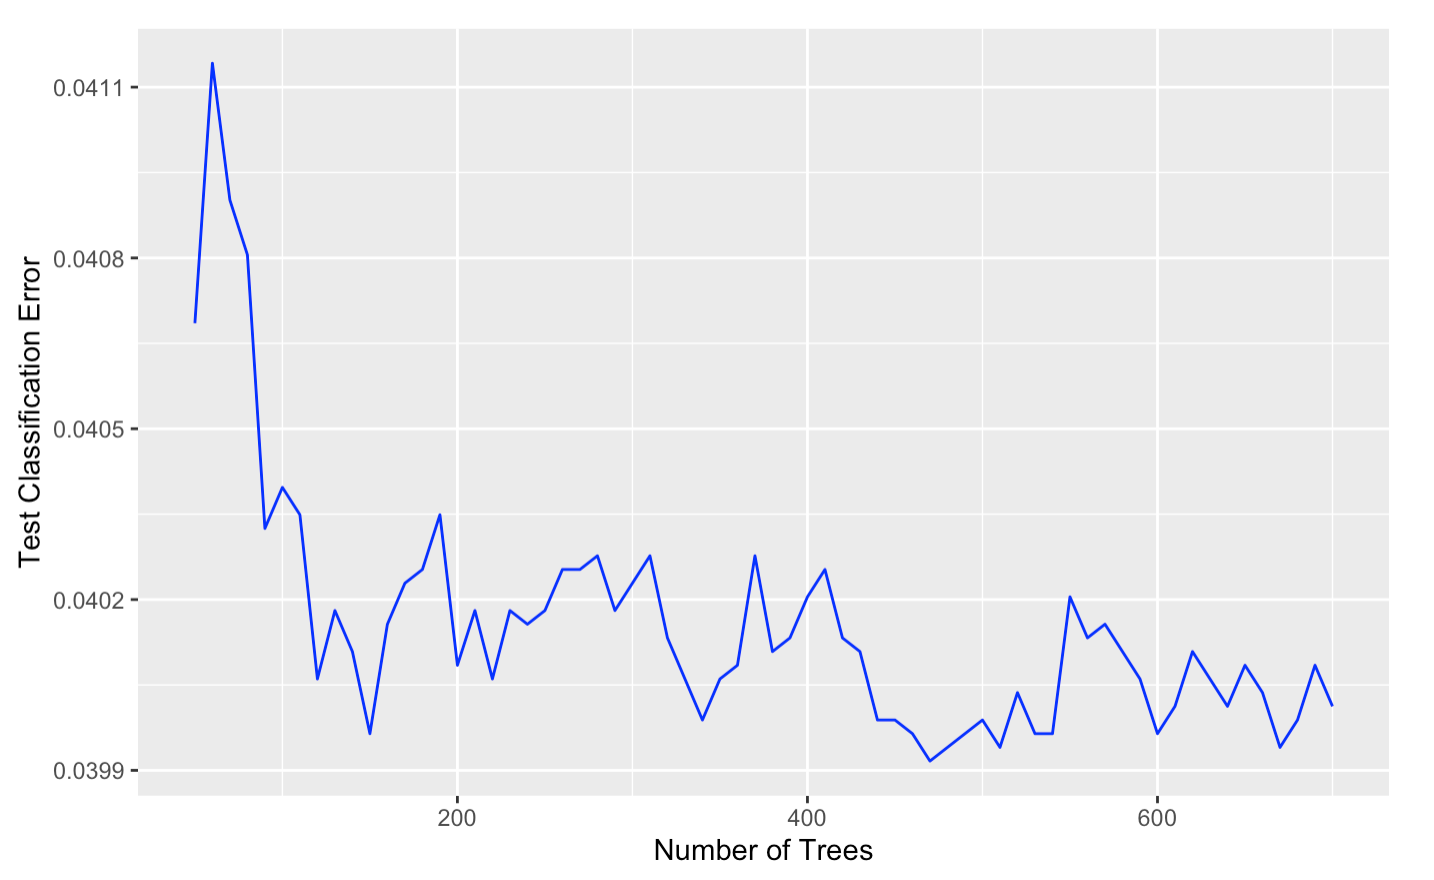
\includegraphics[width=8cm]{figures/4a1.png}
\caption{Undesirable split method}
\label{TCE}
\end{figure}
\FloatBarrier

From the plot, we can see that Random Forest classifier achieves a relatively low test error rate when the number of trees is only around 150. The error rate decreases as the number of trees increases approximately and achieves its lowest at 470, which is smaller than 550 as we previously selected by cross-validation. This difference creates no contradiction since 550 is the number of trees that reaches the best generalization ability, while 470 is the optimal for the particular case. 

Next, we look at the feature importance in the model. Random forests lose straightforward interpretation when compared to decision trees. We can roughly measure which variable is important by calculating the feature importance. Here we use Gini Importance as our feature importance. Gini Importance adds up the total amount that the Gini index is decreased by splits over a given predictor, averaged over all trees. The results are given in Table \ref{gini}.

\begin{table}[h]
    \centering
    \begin{tabular}{c||c|c|c|c|c|c|c|c}

         & NDAI
         & SD
         & CORR
         & DF
         & CF
         & BF
         & AF
         & AN \\
         \hline
         Gini Importance
         & 25375.8
         & 12516.8
         & 14091.7
         & 3565.4
         & 2753.2
         & 3991.1
         & 5918.2
         & 6012.4
    \end{tabular}
    \caption{Gini Importance}
    \label{gini}
\end{table}
\FloatBarrier

The Gini Importance results show that NDAI, SD, and CORR are the three most important features, which have much larger values of Gini Importance than other features. This corresponds to our ``best'' features in section \textbf{2(c)}.

\subsection*{(b)}

We first examine the distributions of the four most important features identified by Gini Importance, namely SD (or $\log$SD), CORR, NDAI, and An. In Figure \ref{4b0}, we could see that

\begin{itemize}
\item For $\log$SD, the distributions for false predictions lie between true predictions, with some overlapping.

\item For CORR, the distribution for true positive is relatively isolated, while the other three overlap quite significantly. This means that higher CORR value could be a decent indicator but the lower value by itself could not quite make the prediction.

\item For NDAI, the distribution for true negative is relatively isolated with generally lower NDAI values, while the other three overlap. Low NDAI value indicates quite well. Our observations for CORR and NDAI agree with the paper in a sense that the paper proposes to combine CORR (greater than some threshold) and NDAI (smaller than some threshold) to predict.

\item For An, the distributions for all categories are not clearly separated, which means An by itself might not be a useful indicator.
\end{itemize}

To summarize, the errors usually occur in the middle range of SD, lower range of CORR, and higher range of NDAI. For other features using zenith angles, errors almost could be made on the entire range since they are not as separable by labels as the three most important features.

\begin{figure}[h]
\centering
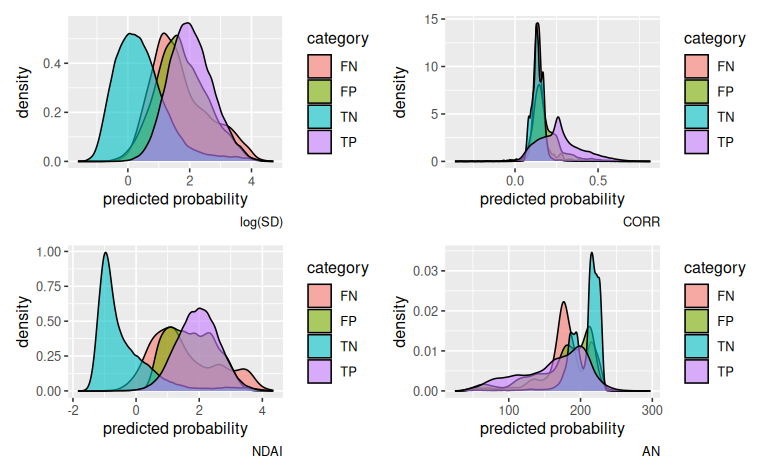
\includegraphics[width=8cm]{figures/4b3.png}
\caption{Distributions of feature values, FN = False Negative, TP = True Positive}
\label{4b0}
\end{figure}
\FloatBarrier

We then proceed to investigate the regions where the misclassification occurs. Figure \ref{4b1K} and \ref{4b1V} illustrates them on the graph, with agree = 1 being correctly classified. We could see that for the training set, they usually occur in the middle range and are surrounded by those that are correctly classified. For the testing set, while some are in the middle range, more likely there would be a cluster of region that are incorrectly classified.

\begin{figure}[h]
\begin{minipage}[t]{0.5\textwidth}
\centering
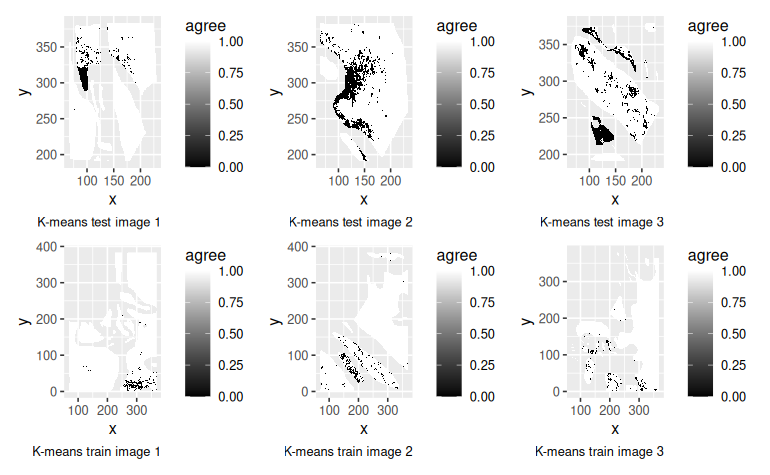
\includegraphics[width=9cm]{figures/4b1K.png}
\caption{Label agreement for $K$-means split}
\label{4b1K}
\end{minipage}
\begin{minipage}[t]{0.5\textwidth}
\centering
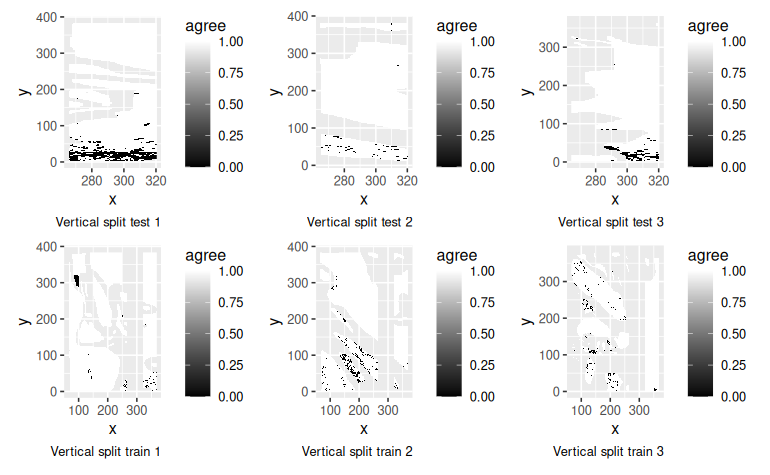
\includegraphics[width=9cm]{figures/4b1V.png}
\caption{Label agreement for vertical split}
\label{4b1V}
\end{minipage}
\end{figure}
\FloatBarrier 

Inspecting the predicted probability output by the Random Forest algorithm suggests that misclassification almost always would occur when the probability assigned is in the middle range. The separability is more prominent in the training set with clear modes.

\begin{figure}[h]
\centering
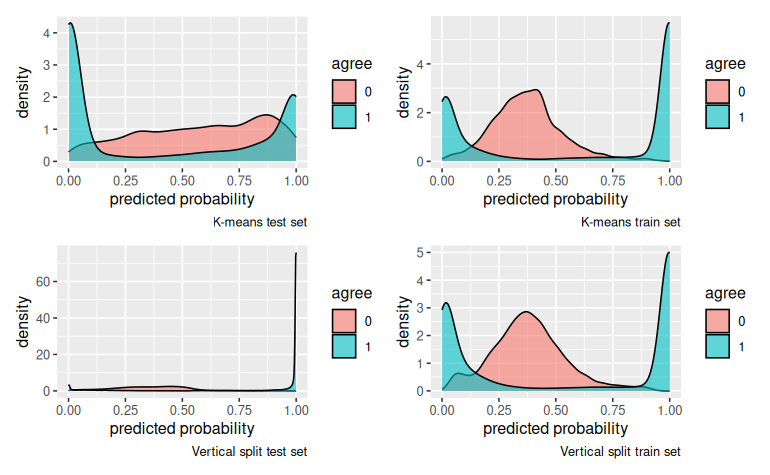
\includegraphics[width=10cm]{figures/4b2.png}
\caption{Predicted probability distributions grouped by agreement}
\label{4b2}
\end{figure}
\FloatBarrier

\subsection*{(c)}
From Figure \ref{4b2}, we found that correctly classified pixels typically are given a predicted probability closed to either 0 or 1. Therefore, we would like to modify our classifier for those pixels that are given ``middle'' values. Also, we notice from Figure \ref{4b1K} and \ref{4b1V} that most of the misclassified pixels in the training set are scattered among large patches of clouds or surfaces (i.e., those misclassified are surrounded by those that are correctly classified). Inspired by the strong spatial dependency that we observed in section \textbf{1(b)}, we would like to modify our classifier in the following way: 

\begin{itemize}
    \item Assign labels to pixels that we are confident with using Random Forest classifier; The confidence probability regions could be set to be $[0, 0.25] \cup [0.75, 1]$ based on Figure \ref{4b2}, or could be set through Cross-Validation and parameter tuning.

    \item Iteratively assign labels to the remaining pixels which are surrounded by several labelled pixels using a $K$-NN classifier (with the exact value of $K$ to be tuned and likely to be based on the size of the image).
\end{itemize}

Note that our new classifier does not work on single pixel classification problem, but works when a relatively complete image is given. This new algorithm is also more efficient compared to implementing $K$-NN classifier throughout. 

Given the predictive power of our three most important features, this model shall work quite well on future data without expert labels. However, we need to be careful when the future input data image contains some "holes" (i.e., a small clear region within a cloud) such that the continuity assumption in section \textbf{1(b)} does not quite hold. In this case, the $K$-NN classifier might not provide the optimal result.

\subsection*{(d)}

From our analysis of Figure \ref{4b2}, we could see that the misclassification behavior for both data splitting methods are similar - with most "middle" predicted probability misclassified. This phenomenon indicates that there is no systematic issue for our data splitting method. A few clusters of misclassification labels in the testing sets are the consequence of "middle" predicted probability instead of the ways how the data is split. It is safe to conclude that both of our splitting methods are valid under this setting.

\subsection*{(e)}
In this report, we attempt to identify an efficient and accurate algorithm to predict the existence of clouds in the Arctic region. Since the input data has some spatial dependency and hence is not identically independently distributed, we apply two different splitting method, $K$-means and vertical split, so that the training, validation, and testing sets could be better separated and allow generalization.

We then implement six different classification algorithms and identify the best model for each via gird search hyper-parameter tuning. Metrics such as ROC curves, F1 scores, and CV errors are used to compare models. Random Forest (with tree number being 550 and tree depth being 15) is eventually selected as it performs well on both splitting method and achieves the minimum average cross-validation error. It also achieves a 95.6\% accuracy on the vertical-split testing set.

Gini importance reveals that NDAI, CORR, and SD are the three most important features in this model. Diagnostic results signals that the misclassification labels in training sets are scattered not clustered in the images, and that those misclassified are predicted with "middle" probabilities. Also, exploratory analysis shows that a pixel surrounded by clouds are almost certain to be a cloud. These observations inspired us to incorporate location information using $K$-NN classifier to predict those pixels with "middle" probabilities. Combining Random Forest and then $K$-NN classifier would likely to produce better results, although cares need to be taken when such "continuity" behavior breaks in future input. Also, another limitation is that $K$-NN only works for input of an image but not on a single pixel.

\section{Reproducibility}
Please refer to README for more information.

\section{Acknowledgement}
The project was jointly developed by Jingan Zhou and Linxuan Wang with equal contribution. In section 1, Jingan completed the half-page summary in \textbf{1(a)} and Linxuan conducted the initial data exploration in \textbf{1(b)} and \textbf{1(c)}. In section 2, Linxuan answered questions in \textbf{2(a), 2(b)} and \textbf{2(c)}. Linxuan and Jingan jointly designed the \textbf{CVmaster} function in \textbf{2(d)}, where Random Forest, Logistic Regression and Naive Bayes classifiers were done by Linxuan; LDA, QDA and XGBoost classifiers were done by Jingan. In section 3, we divided the work in \textbf{3(a), 3(b)} as in \textbf{2(d)}. Jingan completed the bonus question in \textbf{3(c)}. In section 4, Linxuan completed \textbf{4(a)} and designed the classifier in \textbf{4(c)}; Jingan completed \textbf{4(b), 4(d)} and \textbf{4(e)}. Linxuan also had some discussion with Yunhong Bao on how to deal with spatial dependency, which inspired both of them on a better classifier design in \textbf{4(c)}. We mainly referred to the materials in STA 521 lectures and labs.

\end{document}
